
\documentclass[a4paper, 11pt]{article}

\usepackage{verbatim}
\usepackage{pdfpages}
\usepackage[T1]{fontenc}
\usepackage{titling}
\usepackage{amsmath}
\usepackage{siunitx}
\usepackage{amsfonts}
\usepackage{graphicx}
\usepackage{mathtools}
\usepackage[includeheadfoot,margin=23mm]{geometry}
\usepackage{multirow}
\usepackage{siunitx}
\usepackage{mhchem}
\usepackage{xfrac}
\usepackage{epstopdf}
\usepackage{float}
\makeatletter
\newcommand{\sectionauthor}[1]{}
\makeatother
\usepackage[bottom]{footmisc}
\usepackage{helvet}
\renewcommand{\familydefault}{\sfdefault}

\usepackage{chngcntr}
\counterwithin{figure}{section}

\usepackage{caption}
\usepackage{subcaption}

\usepackage{gensymb}

\usepackage{setspace}
\doublespacing

\usepackage{fancyhdr}
\pagestyle{fancy}
\cfoot{\fancyplain{}{\thepage}}

\usepackage{fancyhdr}
\pagestyle{fancy}
\fancypagestyle{wojciech}{
	\fancyhead{} % clear all header fields
	\lhead{\leftmark }
	\rhead{Wojciech Dziwulski}
	\cfoot{\thepage}
}


\usepackage{titlesec}
\setcounter{secnumdepth}{4}
\titleformat{\paragraph}
{\normalfont\normalsize\bfseries}{\theparagraph}{1em}{}
\titlespacing*{\paragraph}
{0pt}{3.25ex plus 1ex minus .2ex}{1.5ex plus .2ex}
\usepackage{gensymb}



\renewcommand{\headrulewidth}{0.5pt}

\numberwithin{equation}{section}
\usepackage[numbered, framed]{matlab-prettifier}

\lstset{
	style              = Matlab-editor,
	escapechar         = ",
	mlshowsectionrules = true,
	tabsize            = 2,
}

\graphicspath{{Images/}}

\setlength{\droptitle}{-8em}

\title{Distributed Neural Network Training \\ \large Final Year Project}

\author{\textbf{Wojciech Dziwulski}}

\date{}

\begin{document}
	
	\clearpage
	\maketitle
	\thispagestyle{empty}
	\begin{abstract}
		 Nothing here yet.
		
	\end{abstract}
	
	
	\newpage
	\pagenumbering{roman}
	\tableofcontents 
	
	
	\newpage
	\pagenumbering{arabic}
	
	
	\clearpage
	

		\newpage
		
		\clearpage
			
		\pagestyle{wojciech}
		
		\section{Introduction}
		
		Understanding data was the cornerstone of humanity's development, its greatest feat and challenge. It is undoubtedly the reason why we become rational beings, even though we come to this world blissfully helpless. Due to the rapid technological revolution of the past few decades we now produce more data than was previously imaginable, and hence develop novel techniques for making sense of it. The data we produce, however, is as diverse as it is abundant, with different data sets requiring very different analysis and treatment. Classifying emails as spam is clearly a task whole lot different than image recognition, which is in turn dissimilar to natural language processing.
		
		For simplicity, let's look at the spam classification example. We can imagine the data as points occupying a multi-dimensional space. The point coordinates describe its features - in our case the occurence of fraudulent clauses, grammar correctness, legitimacy of the email address and many more. Based on those features, we can try to draw a classification boundary - for example a hyperplane dividing the bad from the good, \textbf{to the extent that our algorithm can work it out}. Not every algorithm will come up with the same boundary, though, and only some will come up with a valid one. This depends on the characteristics of the dataset.
		
		The most rudimentary way of describing the interdependencies between variables in the set is their linearity. If we can describe the classification boundary by a function linear in its coefficients, then we call the dataset linear. Most of algorithms can deal with this sort of datasets quite well. In fact, if we extend our discussion to regression problems, the learning problem has already been approached in the 19th century. This is because even fitting a best-fit line to a set of points on a 2D plane lets us detect trends in the data. Problem arises when the dataset is not linearly separable - if there is a more subtle relationship between the data features. Sadly for linear regression, but excitingly for the development of science, most of the "natural" datasets we study are not linear. \textbf{Machine learning} is the field concerned with developing techniques robust to the dataset charasteristics and bringing the technology closer to the sophistication with which the humans understand the world.
		
		Interestingly the problems that we, humans, find awfuly easy, such as informed vision, turn out to be tremendously hard for the computers to perform. Our brains are amazingly sophisticated machines, with the computational power available at a very low energetic cost. Millions of years of evolution equipped us with skills that are impossible to replicate with the current technology, which certainly doesn't mean we shouldn't try, though! The research on human visual cortex (Kruger et al., 2013 \cite{kruger2013deep}), for example, gave us significant insight into the generalised machine vision problems, and stimulated the development of a field known as deep learning. Before we delve into the analysis of deep learning itself, though, it is useful to take a quick look at the algorithm underlying its success - a neural network.
		
		\section{Background - machine intelligence}
		
		\subsection{Neural networks}
		
		\cite{ng2015coursera} It was noted at the end of the previous section that linear regression's most obvious drawback is the inability to cope with non-linear datasets. This is largely due to the fact that expanding the feature set to include the non-linearities (e.g. quadratic cross feature products) would grow the storage space unreasonably. Both random forests and artificial neural networks are in theory able to address that problem. Their inherently non-linear architectures help conforming to more diverse and complex classification challenges. \\
		
		As the name suggests, the artificial neural networks are loosely based on the human brain's intricate internal architecture. Their most basic building block is a logistic unit, which works similarly to a logistic regression classifier.
		
		\begin{figure}[!h]
			\centering
			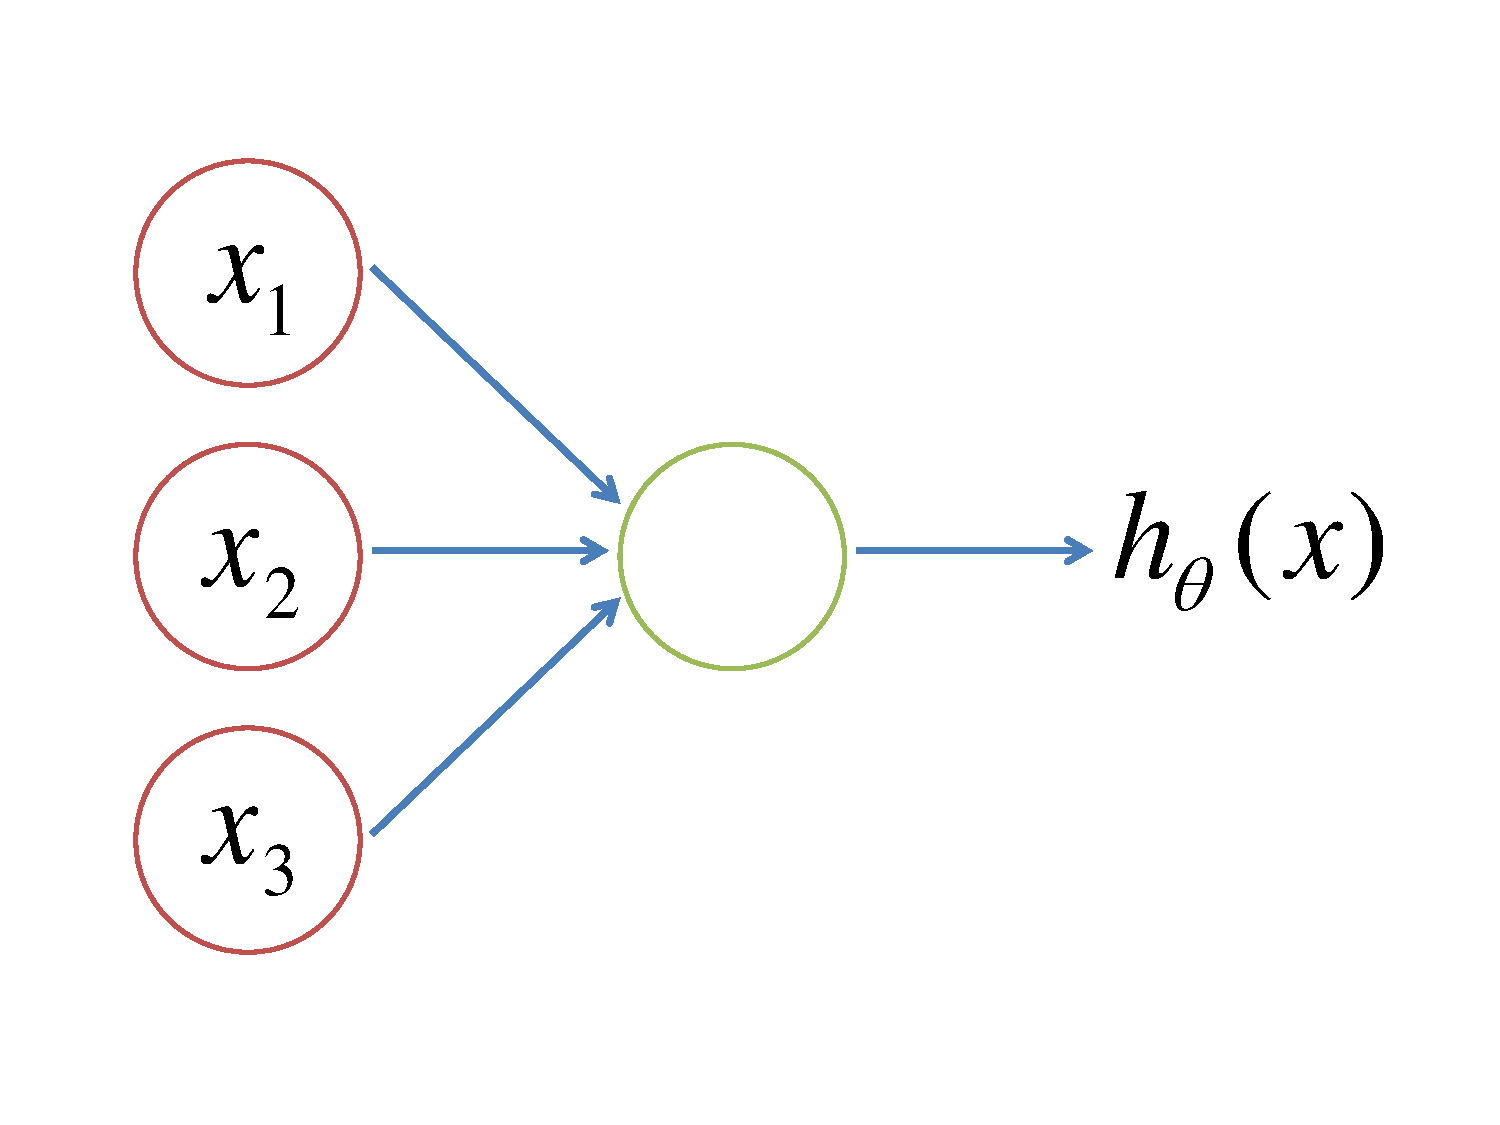
\includegraphics[page=1,width=0.40\textwidth]{logistic_unit.pdf}
			\caption{\label{fig:logistic_unit}{A logistic unit}}
		\end{figure}
		
		The logistic unit takes in input features $x_1, x_2, ..., x_n$ and makes an output decision using a logistic sigmoid function, i.e. (as before):
		
		\begin{equation}
		h_\theta (x) = \frac{1}{1+e^{-\theta ^ T x}}
		\end{equation}
		where $\theta$ are the feature weights.\\
		
		Naturally, many more of those logistic units are combined within a layer of a neural net and many more layers are combined to form a neural network (see fig. \ref{fig:neural_net}). It comprises of one input and one output layer, in addition to several (in case of the aforementioned figure just one) hidden layers. Output is then calculated according to:
		
		\begin{align}
		a_1^{(2)} &= \sigma (\Theta_{10}^{(1)} x_0 + \Theta_{11}^{(1)} x_1  + \Theta_{12}^{(1)} x_2  + \Theta_{13}^{(1)} x_3) \\
		a_2^{(2)} &= \sigma (\Theta_{20}^{(1)} x_0 + \Theta_{21}^{(1)} x_1  + \Theta_{22}^{(1)} x_2  + \Theta_{23}^{(1)} x_3) \\
		a_3^{(2)} &= \sigma (\Theta_{30}^{(1)} x_0 + \Theta_{31}^{(1)} x_1  + \Theta_{32}^{(1)} x_2  + \Theta_{33}^{(1)} x_3) \\
		\Rightarrow h_{\Theta} (x) &= \sigma (\Theta_{10}^{(2)} \boldsymbol{a_0} + \Theta_{11}^{(2)} \boldsymbol{a_1}  + \Theta_{12}^{(2)} \boldsymbol{a_2}  + \Theta_{13}^{(2)} \boldsymbol{a_3})
		\end{align}
		where the superscript denotes the layer number. Or, more compactly:
		\begin{align}
		a^{(2)} = \sigma(\Theta^{(1)} x^{(1)}) \\
		h_{\Theta}(x) = \sigma(\Theta^{(2)} a^{(2)})
		\end{align}
		
		\begin{figure}[!h]
			\centering
			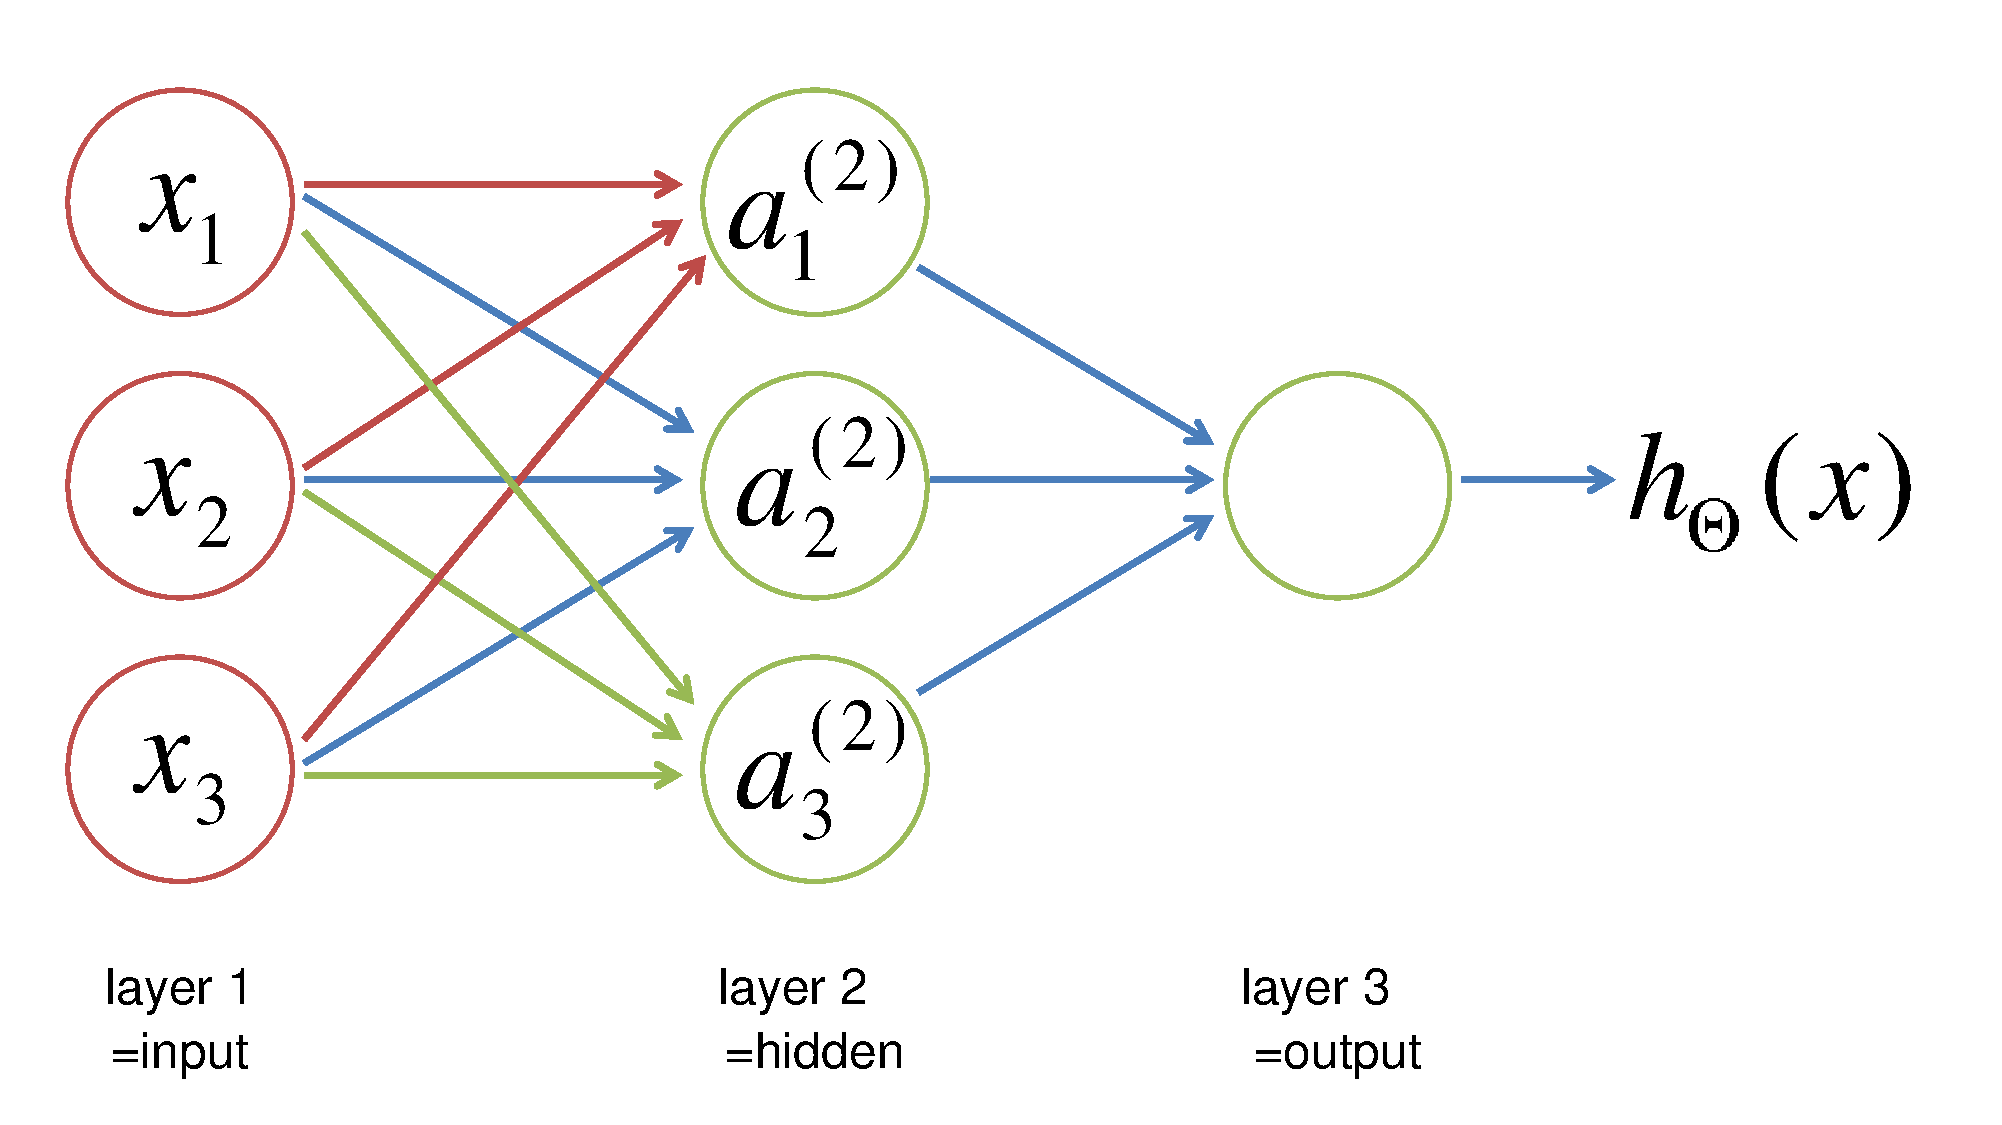
\includegraphics[page=1,width=0.60\textwidth]{neural_net.pdf}
			\caption{\label{fig:neural_net}{A simple neural net}}
		\end{figure}
		
		The computation above is called forward propagation, because it sequentially calculates the activation value $a$ for particular layers of logistic units using the previous ones. Now the most important feature of the neural nets is that the features within the layers (e.g. $a_1^{(2)}, a_2^{(2)}, a_3^{(2)}$) are "learnt" automatically, by appropriately tweaking the $\Theta$ vector using an algorithm called the back propagation.
		
		At the heart of many learning algorithms is minimisation of some kind of a cost function. Neural networks are one such algorithm, where the cost function is defined as:
		\begin{equation}
		J(\Theta) = - \frac{1}{m} \Bigg[\sum_{i=1}^{m} \sum_{k=1}^{K} y_k^{(i)}log(h_\Theta(x^{(i)}))_k + (1-y_k^{(i)}) log(1-(h_\Theta(x^{(i)}))_k) \Bigg] + \frac{\lambda}{2m} \sum_{l=1}^{L-1} \sum_{i=1}^{s_l} \sum_{j=1}^{s_{l+1}} (\Theta _ {ji} ^{(l)})^2
		\end{equation}
		where $l$ is the network layer number, $L$ is the total number of layers, $s_l$ is the number of layers in layer $l$ and $K$ is the number of output units. The second term ($\frac{\lambda}{2m} \ldots$) is a regularization term.
		In order to minimize the cost, we also need to know how to compute the gradient with respect to individual connection weights within the nets i.e.:
		\begin{equation}
		\frac{\partial}{\partial \Theta_{ij}^{(l)}} J(\Theta))
		\end{equation}
		
		That is where the back propagation comes into play. To illustrate its operation, we can assume being given one training example $(x, y)$ for which, using a randomly initialized neural net, we run the first forward propagation sweep to obtain the initial prediction:
		\begin{align}
		a^{(1)} &= x \\
		a^{(2)} &= \sigma(\Theta^{(1)} a^{(1)}) \\
		&\ldots \\
		a^{(L)} &= h_{\Theta}(x)= \sigma(\Theta^{(L-1)} a^{(L-1)})
		\end{align}
		
		Now, starting from the output layer of the net, we can compute the "error", whose value will help us obtain the gradient:
		\begin{align}
		\delta^{(L)} &= a^{(L)} - y \quad \textrm{for the last layer} \\
		\delta^{(L-1)} &= (\Theta ^ {(L-1)})^T \delta^{(L)} \cdot \sigma'(\Theta^{(L-2)} a^{(L-2)}) \\
		&\ldots \\
		\delta^{(2)} &= (\Theta ^ {(2)})^T \delta^{(3)} \cdot \sigma'(\Theta^{(1)} a^{(1)})
		\end{align}
		where $\sigma'$ is the derivative of the logistic sigmoid, which is easily computed as:
		\begin{align}
		\sigma'(\Theta^{(n)} a^{(n)}) = a^{(n+1)} \cdot (1-a^{(n+1)})
		\end{align}
		Now, incidentally, it can be shown that:
		\begin{equation}
		\frac{\partial}{\partial \Theta_{ij}^{(l)}} J(\Theta)) = a_j^{(l)} \delta_i^{(l+1)}
		\end{equation}
		
		Given that we know how to calculate the gradient, we can now try to minimize the cost function using gradient descent. As the number of iterations of back propagation increases, the forward propagation sweeps through the net should yield results closer and closer to the ground truth.
		
		\subsection{Deep learning}
		
		As mentioned before (Kruger at al., 2014 \cite{kruger2013deep}), human visual cortex and deep learning have, or at least are meant to have, a lot in common. Based on the research on the visual cortex, we can characterise the human vision and perception by its structural composition. It is apparent, that the neural structure is hierarchical, in that the visual impulses pass through consecutive stages of processing before identification. The lower "layers" of the cortex distinguish the simple image features over specialised regions and then pass on the information to the higher areas which are able to identify increasingly higher level context of the image.
		
		The technical complexity of the process is supported by the computational efficiency of the structure. The cortical areas share feature recognition information to enable straightforward storage and processing. Because of the hierarchical structure of the visual cortex and the large number of processing layers that are passed before final classification, such structures are called "deep" and are able to achieve tremendous efficiency. This certainly sets a good example for engineering artificials structures used for similar purposes.
		
		The reason why we speak about \textbf{convolutional} nets \cite{stanford2016convnets} is that our artificial neurons are in this case convolutional filters that we apply to the outputs of consecutive neural layers. They are the little windows that we dot product with consecutive areas of the input in order to get an "activation map". Each filter generates an activation map of its own, so combined together they assemble a 3d volume of neuron activations. This first step of the computation is, not surprisingly, called the \textbf{convolutional layer}.
		
		What comes next is the ReLU layer of the \textbf{rectified linear unit}, which might simply be an activation sigmoid function used to threshold the values generated before. 
		The \textbf{pooling layer} performs a downsampling operation on the thresholded set, in order to reduce the order of computation.
		Lastly, as in traditional neural nets, there is  a \textbf{fully-connected layer} which constitutes the last step of classification, whose output corresponds to the identified labels.
		
		Since the depth of the convolutional filter is always equal to the depth of its input, the resulting activation map has unit depth (see fig. \ref{fig:conv_net}). To avoid the curse of dimensionality, or explosion of the parameter space size, we assume that the neurons within one activation map share the same weights and bias i.e. if a filter is useful in one area of the image, it will also be useful in the other. Similarly to traditional neural nets, we then use the back-propagation algorithm in order to adjust the neural weights and bias and eventually train the classifier.
		
		\begin{figure}[!h]
			\centering
			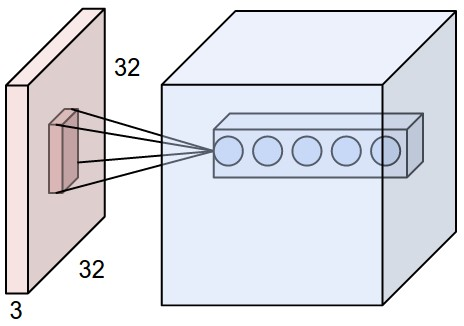
\includegraphics[page=1,width=0.40\textwidth]{depthcol.jpeg}
			\caption{\label{fig:conv_net}{The input volume in red is transformed into a set of 5 activation layers using 5 convolutional filters.}}
		\end{figure} 
		
		\section{Scaling and parallelisation}
		
		It has been proven before (Ciresan et al., 2010 \cite{ciresan2010deep}) that the accuracy of the neural system classification algorithm increases tremendously if large datasets are available. This is consistent with our intuition - the more training examples and the broader the example space, the better we can learn how to replicate the results and correctly classify new data. Even though scaling the datasets is a widely accepted way of improving the classification accuracy, it comes at a significant cost - the time required to train the networks does not expand linearly with the amount of data fed. This poses a significant issue, as the current technology is not capable of training the nets of the desired size. At least not in a linear manner.
		
		Parallel computation is a technique that greatly speeds up the training by breaking down the outstanding training jobs between different cores of a processor or, ideally, different machines. One advancement in the area came with the realisation that a device perfectly suited for parallel computation is the GPU - Graphical Processing Unit. Whereas the CPU is suited perfectly for sequential tasks, the GPU comes second-to-none when there is a lot of smaller tasks to be handled at the same time. It consists of hundreds of small cores which, although originally designed to render graphics, can be succesfully adapted for the parallelisation of deep learning. Interestingly, the hardware vendors responded extensively to the needs of the scientific (and commercial) machine learning community by providing extensive frameworks for GPU programming (e.g. NVIDIA CUDA).
		
		Even though revolutionary, GPUs can be proved to be insufficient for large neural networking training. As mentioned before, the prediction accuracy scales with the model size, and the amount of data we can fit on a single machine with a couple of GPUs is clearly limited. This explains the need for even grater parallelisation - not only between various cores of the GPU itself, but also between various servers. 
		
		\section{Breaking it down}
		\label{breakingitdown}
		
		Efficient parallelisation between servers turns out to be an extremely complicated task. Considerations regarding net partitioning span several areas, for example:
		\begin{enumerate}
		\item Parallelisation within the individual machines
		\item Partitioning architecture
		\item Storage of net parameter weights and activations
		\item Communication of the newly computed values
		\item Updating conflicting results
		\item Optimization algorithms
		\end{enumerate}
		
		There has been several academic attempts at the problem, most notably: "Large Scale Distributed Deep Networks" (Dean et al., 2012 \cite{dean2012large}) and "Project Adam: Building an Efficient and Scalable Deep Learning Training System" (Chilimbi et al., 2014 \cite{chilimbi2014project}). Both of these are described below with respect to their solutions to the enumerated problems.
		
		\subsection{Large Scale Distributed Deep Networks}
		
		The paper focuses on two advencements developed by the authors: a software framework called \textbf{DistBelief} as well as two algorithms: \textbf{Downpour SGD} and \textbf{Sandblaster L-BFGS}. DistBelief can be considered a solution to problems 1-5 listed in section \ref{breakingitdown}, whereas the two algorithms are optimization procedures tailored for the highly distributed network training.
		
		\begin{figure}[H]
		\centering
		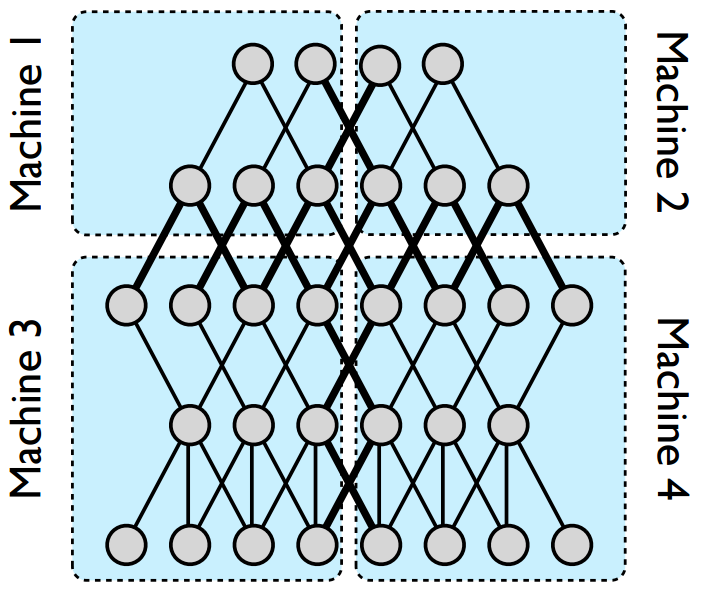
\includegraphics[width=0.40\textwidth]{distbelief.png}
		\caption{\label{fig:distbelief}Example model architecture in DistBelief \cite{dean2012large}}
		\end{figure}
		
		The DistBelief framework is a comprehensive tool that lets the user define the net architecture (fig. \ref{fig:distbelief}) and computation in the chosen nodes. There is no extra user intervention required - the framework takes care of the intra-machine parallelism as well as communication between the machines. Interestingly, splitting the net across several machines does not always yield the most optimal results - it might easily be the case that the communication costs prevail and the overall process is slowed down due to inter-machine parallelism. In addition to communication inefficiencies, different machines will also complete their workload in different time, hence wasting the computational resources and leading to slowdowns.
		
		One of the most common optimization algorithms is Stochastic Gradient Descent. It is extremely versatile and has a myriad of applications, however due to its inherently sequential character it is hard to simply apply it to a highly parallelised problem. The paper hence proposed an asynchronous variant of SGD - Downpour. The training data is broken down and trained on separate copies of the model which run independently of each other. The algorithm is highly randomised, and there is little guarantee the asynchronous parameter updates will be in-order or will not result in data loss. As the authors point out, though, this relaxation brings about effective results. Another improvement is using separate learning rates for various parameters (Adagrad).
		
		An alternative optimization procedure presented in the paper is Sandblaster L-BFGS. As opposed to typical BFGS, the model replicas are assigned much smaller data portions. This mitigates the impact of slow machines, which just process a smaller portion of data in the alloted time, as compared to the better performing units.		 
		
		\subsection{Project Adam}
		
		Project Adam is a framework somewhat resembling the one described above. It also supports the highly parallelised computation, however, as a newer technology, it also offers a couple of improvements.
		
		Adam architecture devotes several machines exclusively for \textbf{data serving}, including the necessary data processing beforehand. In the visual tasks, in order to proliferate the data sets images undergo multiple transformations such as reflections and rotations. Decoupling data serving compute-load from the actual network training specialises the machines in the given tasks and hence speeds up the overall process.
		
		Due to the highly parallelised nature of the framework, there are several characteristics of the architecture that are worth mentioning. First of all, the training on each of the machines is multi-threaded. The threads share the network parameters and, what is more imporant, update them without using locks. This of course implies that the updates are not guaranteed to be based on the latest version of the model, but the training was proven robust enough to converge even in the presence of the noise. As mentioned earlier, the uneven processing times between the machines is a significant bottleneck of the process. Adam architecture tries to mitigate this by finishing an epoch processing after only 75\% of the model replicas have terminated computation.
		
		The shared parameter server is another crucial part of the platform. Due to the high computational demand, it breaks down the model parameters into 1MB shards hashed into storage buckets. This is in contrast to the conventional key-value store.
		
		\subsection{Contrast and conclusions}
		
		The two architectures described in the sections before are very distinct, although they share common problems and hence offer some similar solutions. They have both achieved impressive classification results in the 21k category ImageNet classification task - over 15\% accuracy for DistBelief and stunning 29.8\% for the Adam architecture.
		
		The most important takeaways from the papers are:
		\begin{itemize}
		\item There are two distinct ways of dealing with the slow machine bottleneck. One is to break down the computation into much smaller loads and process them gradually as the machines become available (DistBelief). The other is to finish computation after a fraction of the model replicas have finished processing (Adam). Both speed up the training, although the latter clearly introduces some information loss.
		\end{itemize}
		
		\section{ADMM}
		\label{ADMM}
		
		Alternating Direction Method of Multipliers is an algorithm for solving constrained optimisation problems. It is based on the augmented Lagrangian method, although uses partial updates to achieve the function objective.
		
		The standard Lagrangian method aims to minimise a function $f(x)$ subject to a set of constraints in the form $g_i(x)=0$. We do this by introducing another function $L(x)$ which is a combination of the objective and the constraints like:
		\begin{equation}
		\min_{x} L(x) = f(x) + \boldsymbol{\lambda^T g(x)}
		\end{equation}
		
		where $\lambda$ is a vector of the Lagrange multipliers of the functions $g_i(x)$.\\
		
		In ADMM, we are trying to minize a function of the form:
		\begin{equation}
		\min_{x} L(x) = f(x) + g(x)
		\end{equation}
		
		and to do that we introduce an auxiliary variable $y$, which will help us break the problem down into pieces that are easier to handle. $x$ \& $y$ are dual variables and we will be attempting to minimise the difference between them. We are now facing a constrained optimisation problem of the form:
		\begin{align}
		\min_{x,y} L(x,y) = f(x) + g(y) \\
		\textrm{subject to } x = y \Leftrightarrow x-y=0
		\end{align}
		
		which we can solve using Lagrange multipliers method as:
		\begin{equation}
		\label{ADMM_equation}
		\min_{x,y} \max_{\lambda} L(x,y) + \lambda^T (x-y) + \beta ||x-y||^2
		\end{equation}
		
		where the last term is a regularisation minimising the difference between the dual variables. \\
		
		The alternative direction optimisation now runs as follows:
		\begin{enumerate}
		\item fix $y$, $\lambda$ and $\beta$ and update $x$
		\item fix $x$, $\lambda$ and $\beta$ and update $y$
		\item fix $x$, $y$ and $\beta$ and update $\lambda$
		\item update $\beta$ as $\beta^{t+1}=10 \times \beta^{t}$
		\end{enumerate} 
		
		where the individual updates can be computed using a gradient method such as gradient descent.
		
		\section{ADMM and deep learning}
		
		The presented project is aiming to propose an efficient pipeline for highly parallelised deep network training. We can treat multi-threaded training on multiple cores of the GPU as the first stage of the parallelism, with the next stage being the distribution of the network architecture across several machines. A simple case of such distribution is presented in fig. \ref{fig:dual-training}.
		
		\begin{figure}[!h]
					\centering
					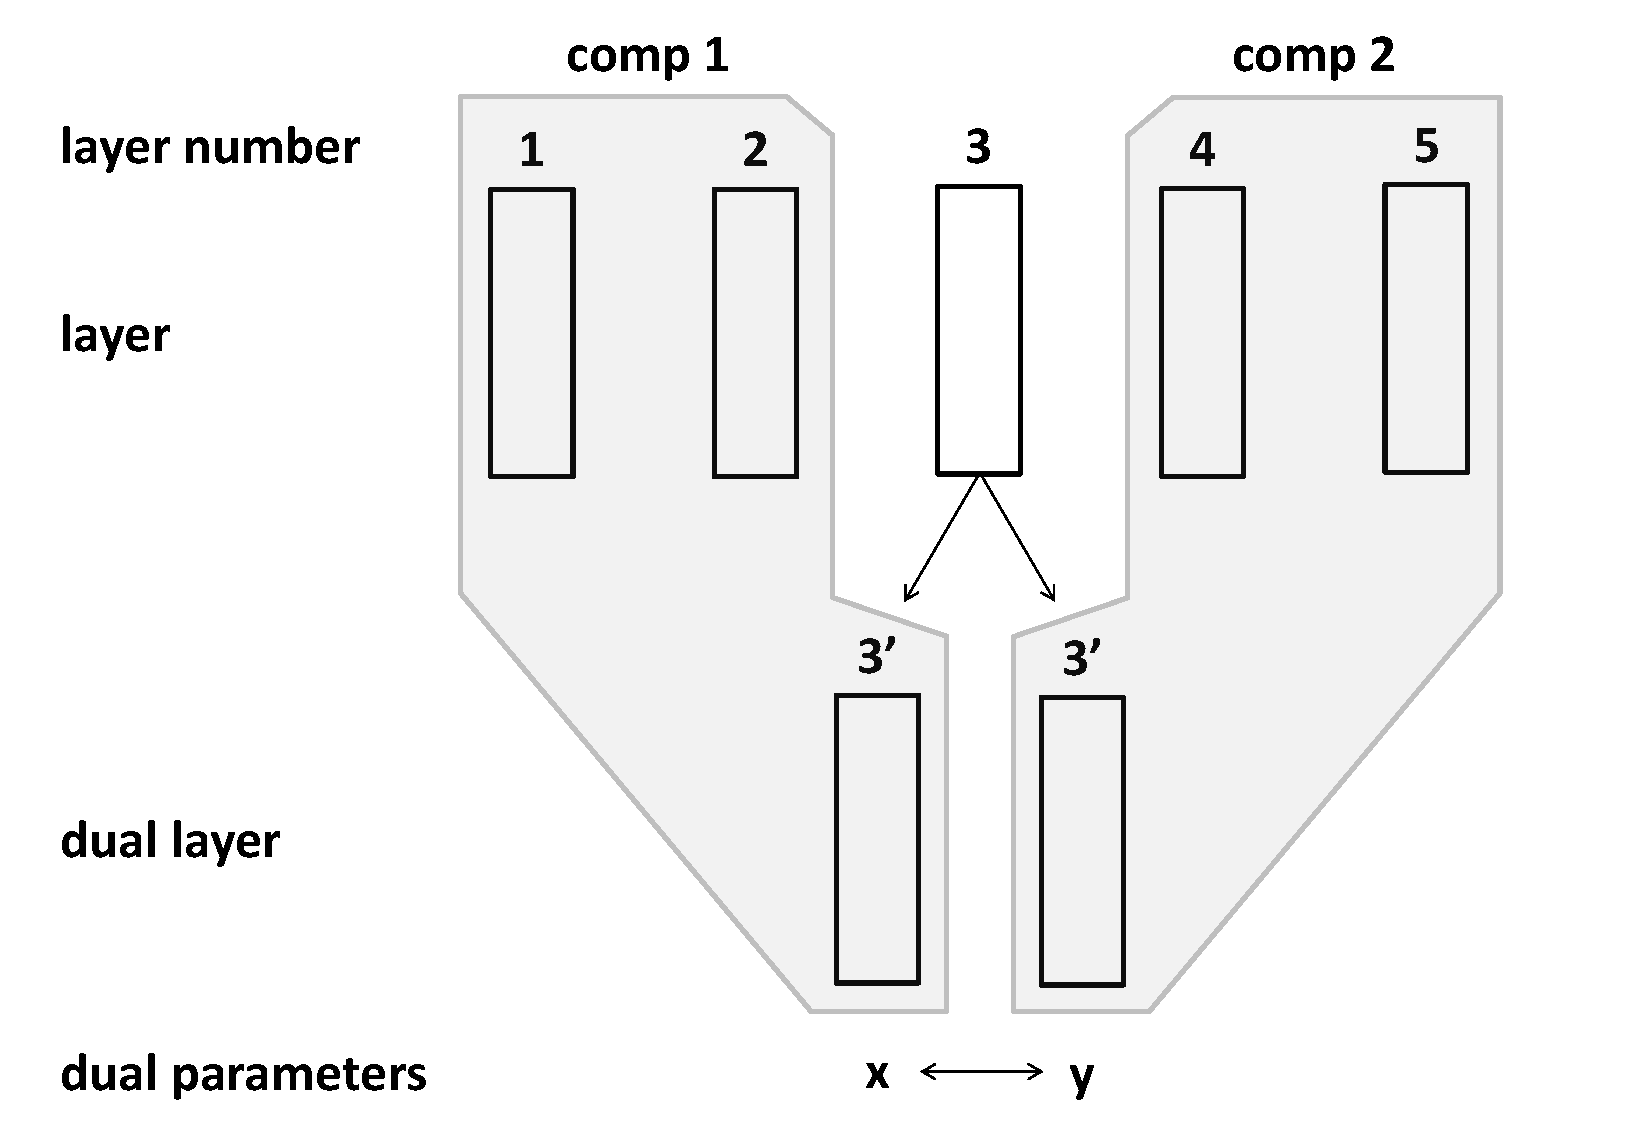
\includegraphics[page=1,width=0.60\textwidth]{dual-training.pdf}
					\caption{\label{fig:dual-training}{Breaking down the network between the machines}}
		\end{figure}
		
		As we can see, the network comprising of five layers is split between two machines: "comp1" and "comp2". The two resulting nets both have 3 layers, with the the highest layer in "comp1" being analogous to the lowest layer in "comp2". The two are deemed as "dual" in the figure, because attempting to minimise the difference between them is a constrained optimisation problem, which in turn can be solved using ADMM (section \ref{ADMM}).
		
		Coming back to the equation \ref{ADMM_equation}, we can see why the two problems are similar. Noting that $\boldsymbol x$ and $\boldsymbol y$ above (the network parameters in the dual layers) can be treated identically to $x$ and $y$ in the equation, ADMM can help us minimise the difference between the two parameter vectors. This in turn will ensure that the distributed neural network training will be convergent to a common set of parameters for the network, albeit computed at separate machines.
		
		\newpage
			
		\clearpage
			
	\newpage
	\pagestyle{plain}
	\bibliography{bib}
	\bibliographystyle{abbrv}

	
\end{document}

